\documentclass[a4paper]{article}
\usepackage{xcolor}
\usepackage{graphicx} % Required for inserting images
\pagecolor{black}
\color{white}
\usepackage{listings}

\title{EE 236 Devices Lab \\ Lab - 03}
\author{Anupam Rawat, 22b3982}
\date{${18^{th}}$ August, 2024}

\begin{document}

\maketitle
\begin{center}
    \section*{Temperature and material dependence of PN diode, IV characteristics}    
\end{center}


\section{Material Dependence}

\subsection{Aim of the experiment}
Simulate the I/V characteristics of silicon (${V_{applied}}$ varies from -5 V to 5 V) \& germanium diodes, using default parameters at 300 K, and plot them. 

\subsection{Silicon and Germanium I/V Characteristic}
\begin{figure}[h!]
    \centering
    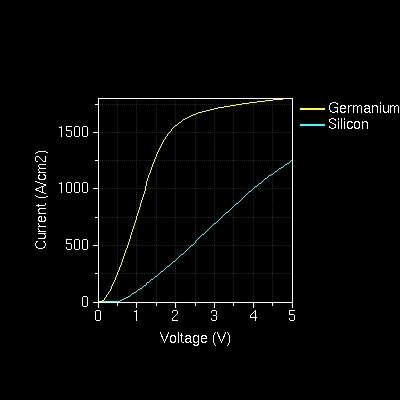
\includegraphics[width=0.7\linewidth]{Lab_3/Part_1_Material_Dependence_linear_scale.png}
    \caption{I/V Characteristic Linear Scale}
\end{figure}

\newpage

\begin{figure}[h!]
    \centering
    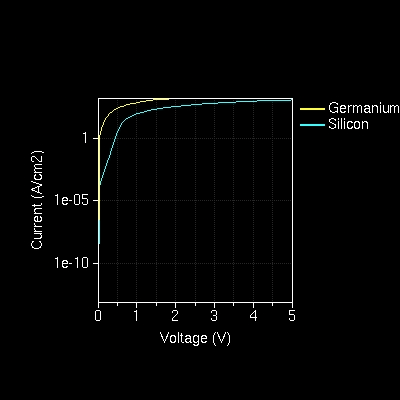
\includegraphics[width=0.7\linewidth]{Lab_3/Part_1_Material_Dependence_log_scale.png}
    \caption{I/V Characteristic Log Scale}
\end{figure}

\subsection{Cut in voltage at 10A/$cm^2$}
\begin{table}[h!]
\centering
\begin{tabular}{|c|c|c|}
\hline
                     & \textbf{Silicon} & \textbf{Germanium} \\ \hline
\textbf{${V_{Cut in}}$} & 0.568 V          & 0.125 V           \\ \hline
\end{tabular}
\caption{Cut-in Voltages for Silicon and Germanium at 10 A/cm\textsuperscript{2}}
\label{tab:cutin_voltages_transposed}
\end{table}

\subsection{Explain the differences in the current densities and the cut-in voltages}
The main difference arises due to difference in the band gap of the two materials. The bandgap of Germanium is 0.66eV while that of Silicon is 1.12 eV. The higher band gap of Silicon causes a higher cut in voltage in Silicon, while the lower band gap of Germanium leads to lower current density of the material's diode.
\newpage
























\newpage

\section{Non Idealities of PN Diode}

\subsection{Aim of the Experiment}
Analyze the non-idealities in the IV characteristics of a silicon PN diode at 300K over a voltage range of 0 to 1.2V. By varying the applied voltage and extracting the ideality factor across different operating regions: recombination (0 - 0.2V), ideal (0.3V - 0.5V), and high injection (0.6V - 0.8V).

\subsection{I/V Characteristics}
\begin{table}[h!]
\centering
\begin{tabular}{|c|c|}
\hline
\textbf{Parameter} & \textbf{Value} \\ \hline
$N_a$ (Acceptor Concentration) & $1 \times 10^{18} \text{ cm}^{-3}$ \\ \hline
$N_d$ (Donor Concentration)     & $1 \times 10^{14} \text{ cm}^{-3}$ \\ \hline
$\tau_{\text{electrons}}$ (Electron Lifetime) & $1 \times 10^{-7} \text{ s}$ \\ \hline
$\tau_{\text{holes}}$ (Hole Lifetime)         & $1 \times 10^{-7} \text{ s}$ \\ \hline
\end{tabular}
\caption{Material Parameters and Carrier Lifetimes}
\label{tab:material_parameters}
\end{table}

\begin{figure}[h!]
    \centering
    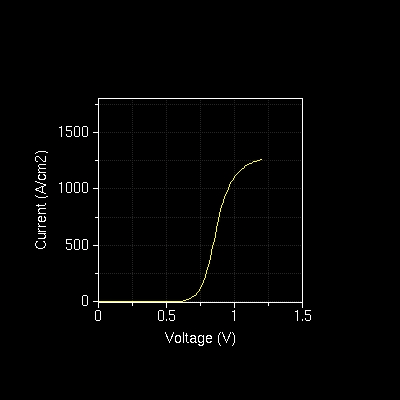
\includegraphics[width=0.7\linewidth]{Lab_3/Part_2_Non_Idealities.png}
\end{figure}

\newpage

\subsection{Ideality Factor Values}
\begin{table}[h!]
    \centering
    \begin{tabular}{|c|c|}
    \hline
    \textbf{Regime}       & \textbf{Ideality Factor (η)} \\ \hline
    Recombination (0 - 0.2V) & 1.363 \\ \hline
    Ideal (0.3V - 0.5V)       & 1.14  \\ \hline
    High Injection (0.6V - 0.8V) & 2.018 \\ \hline
    \end{tabular}
    \caption{Ideality Factors in Different Regimes of a Silicon PN Diode}
    \label{tab:ideality_factors}
\end{table}


\subsection{Reason of Saturation}
The diffusion of minority carriers from neutral regions lead to saturation.




















\newpage
\section{Temperature Dependence}
\subsection{Aim of the experiment}
Simulate the IV characteristics of the silicon diode from 250 K to 400 K, in steps of 25 K

\subsection{Cut in Voltage at !A/$cm^2$}
\begin{table}[h!]
\centering
\begin{tabular}{|c|c|}
\hline
\textbf{Temperature (K)} & \textbf{Cut-in Voltage (V)} \\ \hline
250                      & 0.67                        \\ \hline
275                      & 0.62                        \\ \hline
300                      & 0.56                        \\ \hline
325                      & 0.50                        \\ \hline
350                      & 0.44                        \\ \hline
375                      & 0.38                        \\ \hline
400                      & 0.32                        \\ \hline
\end{tabular}
\caption{Cut-in Voltage as a Function of Temperature for a PN Diode}
\label{tab:cutin_voltage_temperature}
\end{table}

As the temperature increases, the cut in voltage decreases.

\subsection{Band Gap Calculation}
\begin{table}[h!]
\centering
\begin{tabular}{|c|c|c|c|}
\hline
\textbf{Temperature (K)} & \textbf{ln( \( I_{T\text{sat}}^3 \) )} & \textbf{ln(\( I_{\text{sat}} \))} & \textbf{\( \frac{1}{kT} \) (×\(10^{20}\))} \\ \hline
250                      & -39.36438275                            & -22.8                            & 2.90 \\ \hline
275                      & -36.28031329                            & -19.43                           & 2.63 \\ \hline
300                      & -33.47134742                            & -16.36                           & 2.41 \\ \hline
325                      & -30.85147555                            & -13.5                            & 2.23 \\ \hline
350                      & -28.37379946                            & -10.8                            & 2.07 \\ \hline
375                      & -26.06077808                            & -8.28                            & 1.93 \\ \hline
400                      & -23.95439364                            & -5.98                            & 1.81 \\ \hline
\end{tabular}
\caption{Temperature Dependence of \( \ln( I_{T\text{sat}}^3 ) \), \( \ln(I_{\text{sat}}) \), and \( \frac{1}{kT} \) for a PN Diode}
\label{tab:temperature_dependence}
\end{table}

\newpage
Band Gap $E_{g}$ is 0.8865eV

\begin{figure}[h!]
    \centering
    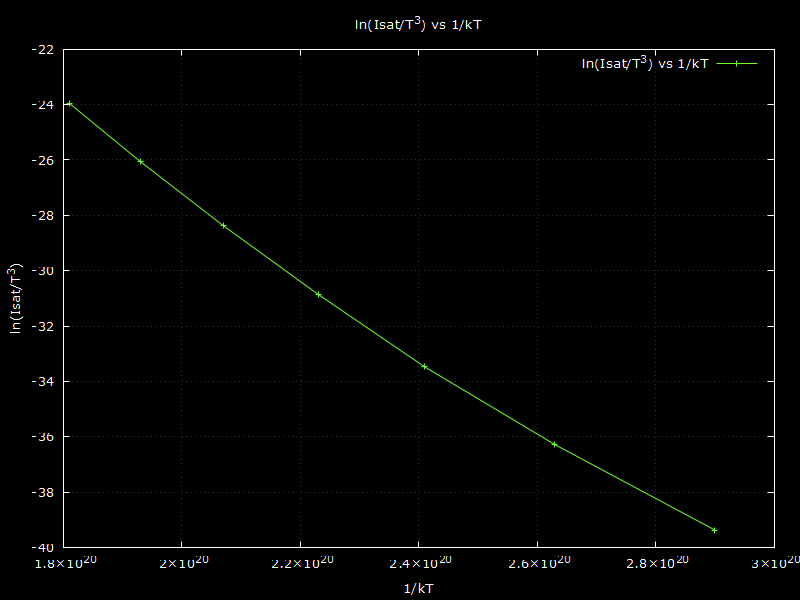
\includegraphics[width=1.3\linewidth]{Lab_3/Part_3_Temperature_Dependance.png}
\end{figure}

\end{document}
